%
% $RCSfile: remote_server.tex,v $
%
% Copyright (C) 2002-2008. Christian Heller.
%
% Permission is granted to copy, distribute and/or modify this document
% under the terms of the GNU Free Documentation License, Version 1.1 or
% any later version published by the Free Software Foundation; with no
% Invariant Sections, with no Front-Cover Texts and with no Back-Cover
% Texts. A copy of the license is included in the section entitled
% "GNU Free Documentation License".
%
% http://www.cybop.net
% - Cybernetics Oriented Programming -
%
% http://www.resmedicinae.org
% - Information in Medicine -
%
% Version: $Revision: 1.1 $ $Date: 2008-08-19 20:41:08 $ $Author: christian $
% Authors: Christian Heller <christian.heller@tuxtax.de>
%

\section{Remote Server}
\label{remote_server_heading}
\index{Remote Server}
\index{Streams}
\index{Common Object Request Broker Architecture}
\index{CORBA}
\index{Simple Object Access Protocol}
\index{SOAP}
\index{Network Dynamic Data Exchange}
\index{NetDDE}
\index{Distributed Component Object Model}
\index{DCOM}
\index{COM+}
\index{KParts}
\index{Universal Network Objects}
\index{UNO}

Figure \ref{remote_figure} introduces a \emph{Remote Server} to the illustrated
example environment. It may access a database system -- similarly to the already
existing application server. In this example, however, it just works on simple
local files, using \emph{Streams}.

\begin{figure}[ht]
    \begin{center}
        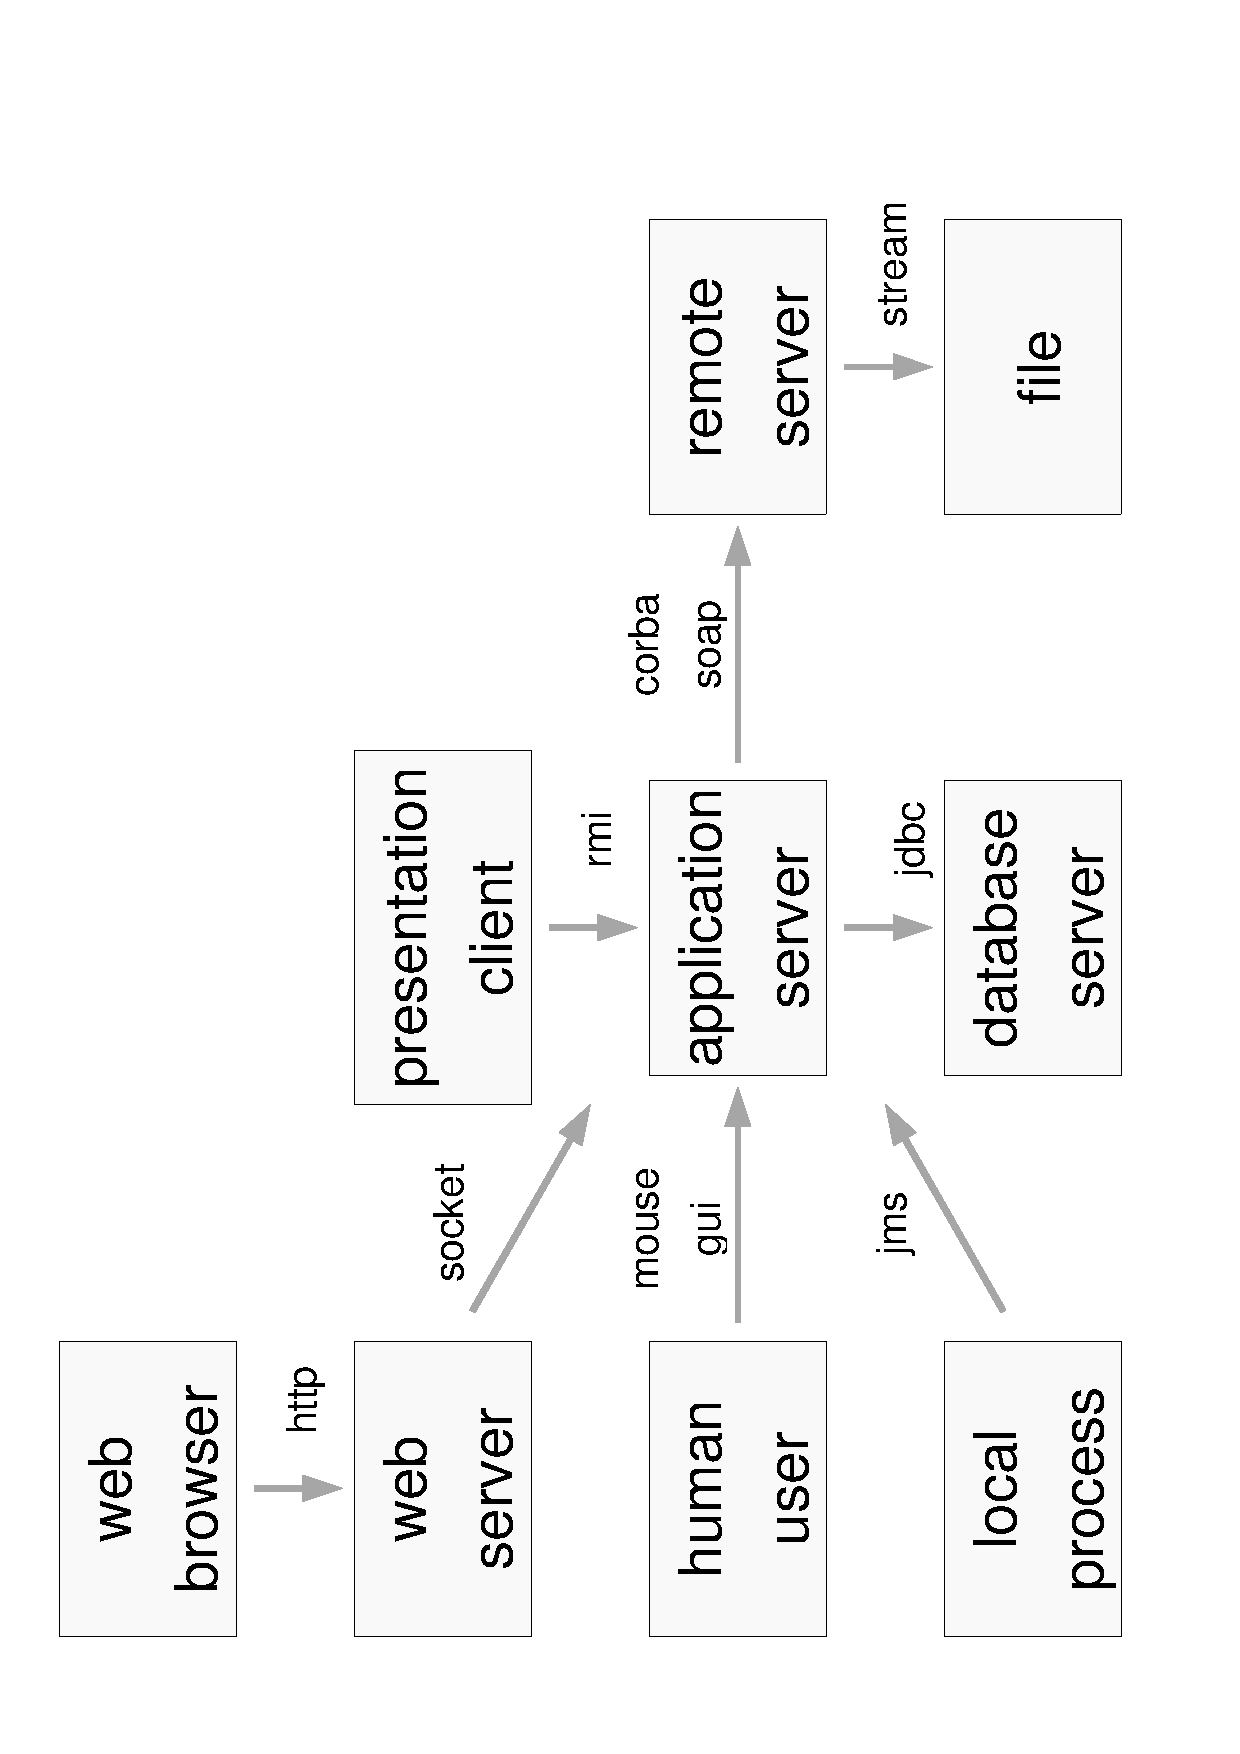
\includegraphics[scale=0.3,angle=-90]{graphic/remote.pdf}
        \caption{Remote Server}
        \label{remote_figure}
    \end{center}
\end{figure}

Like the previously introduced kinds of systems, remote systems need to rely on
a number of standards and mechanisms, in order to be able to communicate over
network. A comparison of some of these is given in \cite{olson, brownech, hrastnik}.
In the following is a list of common techniques that were not yet mentioned
before:

\begin{itemize}
    \item[-] \emph{Common Object Request Broker Architecture} (CORBA)
        \cite{corba, vinoski, gruhn}
    \item[-] \emph{Simple Object Access Protocol} (SOAP) \cite{soap}
    \item[-] \emph{Network Dynamic Data Exchange} (NetDDE) \cite{ddefaq}
    \item[-] \emph{Distributed Component Object Model} (DCOM/ COM+) \cite{gruhn}
    \item[-] \emph{KParts} \cite{kde}
    \item[-] \emph{Universal Network Objects} (UNO) \cite{openoffice}
\end{itemize}
